\documentclass[12pt,letterpaper]{exam}
\usepackage[lmargin=1in,rmargin=1in,tmargin=1in,bmargin=1in]{geometry}
\usepackage{../style/exams}

% -------------------
% Course & Exam Information
% -------------------
\newcommand{\course}{MAT 308: Exam 2}
\renewcommand{\term}{Fall -- 2022}
\newcommand{\examdate}{11/18/2022}
\newcommand{\timelimit}{`$\infty$' Minutes}

\setbool{hideans}{false} % Student: True; Instructor: False

% -------------------
% Content
% -------------------
\begin{document}

\examtitle
\instructions{Write your name on the appropriate line on the exam cover sheet. This exam contains \numpages\ pages (including this cover page) and \numquestions\ questions. Check that you have every page of the exam. Answer the questions in the spaces provided on the question sheets. Be sure to answer every part of each question and show all your work. If you run out of room for an answer, continue on the back of the page --- being sure to indicate the problem number.} 
\scores
\bottomline
\newpage

% ---------
% Questions
% ---------
\begin{questions}

% Question 1
\newpage
\question[10] Consider the `rule' $f: \mathbb{R} \to \mathbb{R}^2$ given by $t \mapsto (3\cos t, 3\sin t)$.
	\begin{enumerate}[(a)]
	\item Is $f(t)$ a function? Explain.
	\item Consider $\im f \subseteq \mathbb{R}^2= \{ (x, y) \colon x, y \in \mathbb{R} \}$. If $(x, y) \in \im f$, show that $x^2 + y^2= 9$. 
	\item Considered as a subset of $\mathbb{R}^2$, geometrically describe $\im f$. 
	\item Can $\im f$ be given by the image of a function of $x$? What about a function of $y$? Explain. 
	\end{enumerate} \pspace

\sol {\itshape
\begin{enumerate}[(a)]
\item Yes, $f(t)$ is a function. For each input $t \in \mathbb{R}$, we have one output---namely, $f(t)= (3 \cos t, 3 \sin t) \in \mathbb{R}^2$. While $\cos t$ and $\sin t$ may be $2\pi$-periodic, $2\pi$ translations of $t$ would be different inputs. For example, $f(0)$ and $f(2\pi)$ have the same value as $f(0)= (3 \cos 0, 3 \sin 0)= (3, 0)$ and $f(2\pi)= (3 \cos 2\pi, 3 \sin 2\pi)= (3, 0)$ but $f(0)$ and $f(2\pi)$ are still well defined because the inputs are different.\pspace

\item Suppose $\mathbf{v} \in \im f \subseteq \mathbb{R}^2$. As $\mathbf{v} \in \mathbb{R}^2$, we know $\mathbf{v}= (x, y)$ for some $x, y \in \mathbb{R}^2$. But because $\mathbf{v} \in \im f$, we know that $\mathbf{v}= (3 \cos t, 3 \sin t)$ for some $t \in \mathbb{R}$. But then using the fact that $\cos^2 \theta + \sin^2 \theta= 1$ for all $\theta \in \mathbb{R}$, we have\dots
	\[
	\begin{aligned}
	x^2 + y^2&= (3 \cos t)^2 + (3 \sin t)^2 \\
	&= 9 \cos^2 t + 9 \sin^2 t \\
	&= 9( \cos^2 t + \sin^2 t) \\
	&= 9 \cdot 1 \\
	&= 9
	\end{aligned}
	\]

\item Observe that elements of $\im f$ satisfy the relation $x^2 + y^2= 9$. Geometrically, as a subset of the plane, $x^2 + y^2= 9$ is a circle of radius 3 centered at the origin. This shows that $\im f$ must be a subset of this circle. The converse is true as well (though it is less immediate). Therefore, $\im f$ is the circle of radius 3 centered at the origin. 
	\[
	\fbox{
	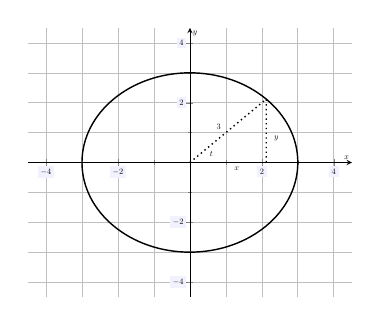
\begin{tikzpicture}[scale=0.6,every node/.style={scale=0.5}]
	\begin{axis}[
	grid=both,
	axis lines=middle,
	ticklabel style={fill=blue!5!white},
	xmin= -4.5, xmax=4.5,
	ymin= -4.5, ymax=4.5,
	xtick={-10,-8,-6,-4,-2,0,2,4,6,8,10},
	ytick={-10,-8,-6,-4,-2,0,2,4,6,8,10},
	minor tick = {-10,-9,...,10},
	xlabel=\(x\),ylabel=\(y\),
	]
	\draw[line width=0.03cm] (0,0) circle (3);
	\draw[line width=0.03cm,dotted] (0,0) -- (2.12132, 2.12132) -- (2.12132,0);
	\node at (0.6,0.3) {$t$};
	\node at (0.8,1.2) {$3$};
	\node at (1.3, -0.2) {$x$};
	\node at (2.4, 0.8) {$y$};
	\end{axis}
	\end{tikzpicture}
	}
	\]
[Note: To see the converse, draw a ray at the angle $t \in \mathbb{R}$, measured from the positive $x$-axis counterclockwise, and let $(x, y)$ be the point of intersection of this ray with the circle. Clearly, $x^2 + y^2= 9$. But using trigonometry, we see that $\cos t= \frac{x}{3}$ and $\sin t= \frac{y}{3}$. This implies $x= 3\cos t$ and $y= 3 \sin t$. Because each such point on the circle can be obtained this way, we can see that every point on the circle has the form $(3\cos t, 3\sin t)$ for some $t \in \mathbb{R}$.]

\item Using (c), we can see that $\im f$ is a circle with radius 3 centered at the origin. But then clearly $\im f$ cannot be a function of $x$ because the circle fails the vertical line test; that is, there are different $x$-values corresponding to the same $y$-value (as shown below). Furthermore, the circle fails the horizontal line test, so that the circle cannot be a function of $y$; that is, there are different $y$-values corresponding to the same $x$-value. \pspace

Alternatively, we can find distinct $x$-values associated to the same $y$-value to show that $f(t)$ is not a function of its $x$-coordinate. Observe that $f \big( \frac{\pi}{2} \big)= (0, 3)$ and $f \big(-\frac{\pi}{2} \big)= (0, -3)$. But then $0 \sim 3$ and $0 \sim -3$ so that $f(t)$ cannot be a function of its $x$-coordinate. Observe also that $f(0)= (3, 0)$ and $f(\pi)= (-3, 0)$. But then $0 \sim 3$ and $0 \sim -3$ so that $f(t)$ cannot be a function of its $y$-coordinate. \pspace

Putting (a)--(d) together, we observe that the circle with radius 3 centered at the origin is neither a function of $x$ or $y$, but it is a function of something---namely, $t$ (its angles). 
\end{enumerate}
}



% Question 2
\newpage
\question[10] Define functions $f, g: \mathbb{R} \to \mathbb{R}$ by $f(x)= |x + 5|$ and $g(x)= 7 - 3x$.
	\begin{enumerate}[(a)]
	\item Find an element in $\im f$ and also find an element in $\im g$. 
	\item Is $-5 \in \im f$? If not, explain why, and if so, find its preimage. 
	\item Is $12 \in \im g$? If not, explain why, and if so, find its preimage. 
	\item Compute $f\big( [-6, 6) \big)$ and $g\big( (-6, 6] \big)$. 
	\item Compute $f^{-1} \big( [-1,1] \big)$ and $g^{-1} \big( [-1, 1] \big)$.
	\end{enumerate} \pspace

\sol {\itshape 
\begin{enumerate}[(a)]
\item Given any $x \in \mathbb{R}$, we know that $f(x)$ and $g(x)$ are elements in the image of $f$ and $g$, respectively. For instance, choosing $x= 0$, we have\dots
	\[
	\begin{aligned}
	f(0)&= |0 + 5|= |5|= 5 \\[0.3cm]
	g(0)&= 7 - 3(0)= 7 - 0= 7 
	\end{aligned}
	\]
Therefore, we have $5 \in \im f$ and $7 \in \im g$. Of course, we need not have chosen $x= 0$, chosen $x$ to be an integer, nor chosen the same $x$-value for both. For instance, we also have\dots
	\[
	\begin{aligned}
	f \left( -\dfrac{11}{2} \right)&= \left| -\dfrac{11}{2} + 5 \right|= \left| -\dfrac{1}{2} \right|= \dfrac{1}{2} \\[0.3cm]
	g(\pi)&= 7 - 3\pi 
	\end{aligned}
	\]
This shows that $\frac{1}{2} \in \im f$ and $7 - 3\pi \in \im g$. \pspace

\item If $-5 \in \im f$, then there is $x \in \mathbb{R}$ such that $f(x)= -5$. But then $|x + 5|= -5$. Because $|x + 5| \geq 0$ for all $x \in \mathbb{R}$, there is no such $x$. Therefore, $-5 \notin \im f$. \pspace

\item If $12 \in \im g$, then there is $x \in \mathbb{R}$ such that $g(x)= 12$. But then\dots
	\[
	\begin{aligned}
	g(x)&= 12 \\
	7 - 3x&= 12 \\
	-3x&= 5 \\
	x&= -\dfrac{5}{3}
	\end{aligned}
	\]
Of course, this only shows that if $g(x)= 12$, then $x= -\frac{5}{3}$. We need show that $g(-5/3)= 12$. This is routine: $g \left(-\frac{5}{3} \right)= 7 - 3 \cdot -\frac{5}{3}= 7 + 5= 12$. Therefore, $12 \in \im g$. \pspace

\item Observe that if $x + 5 \geq 0$, i.e. $x \geq -5$, then $f(x)= |x + 5|= x + 5$. If $x + 5 < 0$, i.e. $x < -5$, then $f(x)= |x + 5|= -(x + 5)= -x - 5$. But then using the fact that if $f(x)$ is a function and $A, B$ are sets that $f(A \cup B)= f(A) \cup f(B)$, we have\dots
	\[
	f \big( [-6, 6) \big)= f \big( [-6, -5] \cup [-5, 6) \big)= f \big([-6, -5] \big) \cup f \big( [-5, 6) \big)= [0, 1] \cup [0, 11)= [0, 11)
	\]
Observe that $g(x)$ is linear because it is of the form $y= mx + b$ with $y= g(x)$, $x= x$, $m= -3$, and $b= 7$. Because $g(x)$ is continuous, it must take intervals to intervals, i.e. the image of an interval is an interval.  Because $m= -3 < 0$, the function is decreasing. Putting these facts together, we know that $g([a, b])= [g(b), g(a)]$, $g \big( (a, b) \big)= \big( g(b), g(a) \big)$, etc. But then we have\dots
	\[
	g\big( (-6, 6] \big)= (g(6), g(-6)]= (-11, 25]
	\]

\item Observe that if $x + 5 \geq 0$, i.e. $x \geq -5$, then $f(x)= |x + 5|= x + 5$. But then if $f(x)= c$ and $x \geq -5$, we have $c= f(x)= |x + 5|= x + 5$ so that $x= c - 5$. Clearly, this then holds if $x= c - 5 \geq -5$, i.e. $c \geq 0$. Now if $x + 5 < 0$, i.e. $x < -5$, then $f(x)= |x + 5|= -(x + 5)$. But then if $f(x)= c$ and $x < -5$, we have $c= f(x)= |x + 5|= -(x + 5)$. But then we have $x= -c - 5$. Clearly, this then holds if $x= -c - 5 < -5$, i.e. $-c < 0$, which of course implies $c > 0$. Putting these two facts together, if $f(x)= |x + 5|= c \geq 0$, then either $x= c - 5$ or $x= -c - 5$. We can check: if $x= c - 5$, then $f(x)= |(c - 5) + 5|= |c|= c$, and if $x= -c - 5$, then $f(x)= |(-c - 5) + 5|= |-c|= c$. But this then shows that if $c \geq 0$, then $f^{-1}(c)= \{ -c - 5, c - 5 \}$. Clearly, $f(x)= |x + 5| \geq 0$ so that if $c < 0$, then $f(x) \neq c$ for all $x \in \mathbb{R}$, i.e. $f^{-1}(c)= \varnothing$. Using these facts and the fact that $f^{-1}$ is the preimage of a function $f$ and $A, B$ are sets, then $f^{-1}(A \cup B)= f^{-1}(A) \cup f^{-1}(B)$, we have\dots	
	\[
	f^{-1} \big( [-1,1] \big)= f^{-1} \big( [-1,0) \big) \cup f^{-1} \big( [0, 1] \big)= \varnothing \cup \big( [-6, -5] \cup [-5, -4] \big)= [-6, -4]
	\]
Observe that if $g^{-1}(c)= x$, then $g(x)= c$. But then $7 - 3x= c$, which implies that $-3x= c - 7$ so that $x= \frac{c - 7}{-3}= \frac{7 - c}{3}$. By the work in (d), because $g(x)$ is a decreasing linear function, the preimage of an interval must be an interval and $g^{-1} \big( (a, b) \big)= \big( g^{-1}(b), g^{-1}(a) \big)$, $g^{-1} \big( [a, b] \big)= \big[ g^{-1}(b), g^{-1}(a) \big]$, etc. But then we have\dots
	\[
	g^{-1} \big( [-1, 1] \big)= \big[ g^{-1}(1), g^{-1}(-1) \big]= \left[ \dfrac{7 - 1}{3}, \dfrac{7 - (-1)}{3} \right]= \left[\; 2, \;\dfrac{8}{3}\; \right]
	\]
\end{enumerate}
}



% Question 3
\newpage
\question[10] Define the function $f: \mathbb{R} \to \mathbb{R}$ via $x \mapsto x^2 + 5$. 
	\begin{enumerate}[(a)]
	\item Is $f(x)$ an injective function? If it is injective, explain why; if it is not injective, give a counterexample. 
	\item Is $f(x)$ a surjective function? If it is surjective, explain why; if it is not surjective, give a counterexample. 
	\item Is $f(x)$ a bijective function? Explain. 
	\item Does $f(x)$ have an inverse function? Explain. 
	\end{enumerate} \pspace

\sol {\itshape 
\begin{enumerate}[(a)]
\item The function $f(x)$ is not injective. If $f(x)$ is not injective, then there exist $x, y$ with $x \neq y$ but $f(x)= f(y)$. Observe that if $x= -1$ and $y= 1$, we have $f(-1)= (-1)^2 + 5= 1 + 5= 6$ and $f(1)= 1^2 + 5= 1 + 5= 6$. But then $f(-1)= f(1)$ but $-1 \neq 1$. Therefore, $f(x)$ is not injective. In fact, if $c \in \mathbb{R}$ and $c \neq 0$, then $f(-c)= f(c)$ but $c \neq -c$: $f(-c)= (-c)^2 + 5= c^2 + 5$ and $f(c)= c^2 + 5$ but we cannot have $c= -c$ because then $2c= 0$ so that $c= 0$, which is impossible if $c \neq 0$. Alternatively, we can see that $f(x)$ is not injective because it fails the horizontal line test: not every horizontal line intersects the function at most once
	\[
	\fbox{
	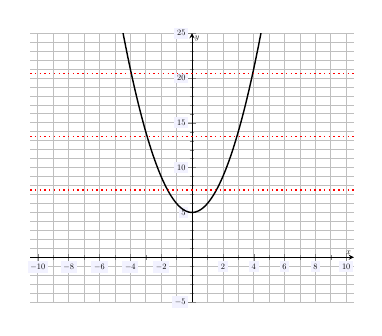
\begin{tikzpicture}[scale=0.6,every node/.style={scale=0.5}]
	\begin{axis}[
	grid=both,
	axis lines=middle,
	ticklabel style={fill=blue!5!white},
	xmin= -10.5, xmax=10.5,
	ymin= -5, ymax=25,
	xtick={-10,-8,-6,-4,-2,0,2,4,6,8,10},
	ytick={-5,0,...,25},
	minor tick = {-25,-24,...,25},
	xlabel=\(x\),ylabel=\(y\),
	]
	\addplot[samples=100,line width=0.03cm] (x, x^2 + 5);
	\draw[line width= 0.03cm, dotted, red] (-10.5, 20.5) -- (10.5, 20.5);
	\draw[line width= 0.03cm, dotted, red] (-10.5, 13.5) -- (10.5, 13.5);
	\draw[line width= 0.03cm, dotted, red] (-10.5, 7.5) -- (10.5, 7.5);
	\end{axis}
	\end{tikzpicture}
	}
	\]

\item The function $f(x)$ is not surjective. If $f(x)$ is not surjective, then there is $c \in \mathbb{R}$ such that $f(x) \neq c$ for all $x \in \mathbb{R}$. Let $c= 4$. If there were $x \in \mathbb{R}$ such that $f(x)= 4$, then we have\dots
	\[
	\begin{aligned}
	f(x)&= 4 \\
	x^2 + 5&= 4 \\
	x^2&= -1
	\end{aligned}
	\]
But if $x \in \mathbb{R}$, then $x^2 \geq 0$. Therefore, there is no $x \in \mathbb{R}$ such that $x^2= -1$. Therefore, $f(x)$ is not surjective. In fact, let $c < 5$. If there were $x \in \mathbb{R}$ such that $f(x)= c$, then we have\dots
	\[
	\begin{aligned}
	f(x)&= c \\
	x^2 + 5&= c \\
	x^2&= c - 5
	\end{aligned}
	\]
But because $c < 5$, we know that $c - 5 < 0$. But because $x^2 \geq 0$, if $x \in \mathbb{R}$, then clearly $x^2 \neq c - 5 < 0$. But then there is no such $x \in \mathbb{R}$ with $f(x)= c$ if $c < 5$. Alternatively, we can see that $f(x)$ is not surjective because not every horizontal line intersects the function at least once.
	\[
	\fbox{
	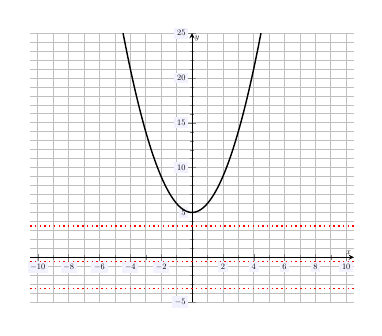
\begin{tikzpicture}[scale=0.6,every node/.style={scale=0.5}]
	\begin{axis}[
	grid=both,
	axis lines=middle,
	ticklabel style={fill=blue!5!white},
	xmin= -10.5, xmax=10.5,
	ymin= -5, ymax=25,
	xtick={-10,-8,-6,-4,-2,0,2,4,6,8,10},
	ytick={-5,0,...,25},
	minor tick = {-25,-24,...,25},
	xlabel=\(x\),ylabel=\(y\),
	]
	\addplot[samples=100,line width=0.03cm] (x, x^2 + 5);
	\draw[line width= 0.03cm, dotted, red] (-10.5, 3.5) -- (10.5, 3.5);
	\draw[line width= 0.03cm, dotted, red] (-10.5, -0.5) -- (10.5, -0.5);
	\draw[line width= 0.03cm, dotted, red] (-10.5, -3.5) -- (10.5, -3.5);
	\end{axis}
	\end{tikzpicture}
	}
	\] \pspace

\item The function $f(x)$ is not bijective. By definition, a function is bijective if and only if it is injective and surjective. By (a), we know that $f(x)$ is not injective. Furthermore, by (b), we know $f(x)$ is not surjective. Therefore, $f(x)$ is not bijective. \pspace

\item The function $f(x)$ does not have an inverse. A function $f: A \to B$ has an inverse function $f^{-1}: B \to A$ if and only if it is a bijection. By (c), we know that $f(x)$ is not a bijection. Therefore, $f(x)$ does not have an inverse function. 
\end{enumerate}
}



% Question 4
\newpage
\question[10] A \textit{fixed point} for a function $f: \mathbb{R} \to \mathbb{R}$ is $x_0 \in \mathbb{R}$ such that $f(x_0)= x_0$. 
	\begin{enumerate}[(a)]
	\item Show that $-5$ is a fixed point for $f(x)= 3x + 10$.
	\item Show that $4$ is not a fixed point for $g(x)= \dfrac{x + 4}{2 - x}$.
	\item Find the fixed points for $h(x)= 2x^2 + 6x - 3$. 
	\item Use the quadratic formula to show that $j(x)= x^2 - 3x + 5$ has no fixed points in $\mathbb{R}$ but does have fixed points in $\mathbb{C}$. 
	\end{enumerate} \pspace

\sol {\itshape
\begin{enumerate}[(a)]
\item If $-5$ is a fixed point for $f(x)$, then $f(-5)= -5$. We check this:
	\[
	f(-5)= 3(-5) + 10= -15 + 10= -5
	\] \pspace

\item If $4$ is not a fixed point for $g(x)$, then $g(4) \neq 4$. We check this:
	\[
	g(4)= \dfrac{4 + 4}{2 - 4}= \dfrac{8}{-2}= -4
	\]

\item If $x$ is a fixed point for $h(x)$, then $h(x)= x$. But then we have\dots
	\[
	\begin{aligned}
	h(x)&= x \\
	2x^2 + 6x - 3&= x \\
	2x^2 + 5x - 3&= 0 \\
	(2x - 1)(x + 3)&= 0 
	\end{aligned}
	\]
But then either $2x - 1= 0$, which implies $x= \frac{1}{2}$, or $x + 3= 0$, which implies $x= -3$. Of course, this only shows that if $x$ is a fixed point, then $x= \frac{1}{2}$ or $x= -3$. This does not necessarily imply that $h \left( \frac{1}{2} \right)= \frac{1}{2}$ or $h(-3)= -3$. We need check this:
	\[
	\begin{aligned}
	h \left( \frac{1}{2} \right)&= 2 \left( \dfrac{1}{2} \right)^2 + 6 \cdot \dfrac{1}{2} - 3= \dfrac{1}{2} + 3 - 3= \dfrac{1}{2} \\[0.3cm]
	h(-3)&= 2(-3)^2 + 6(-3) - 3= 18 - 18 - 3= -3 
	\end{aligned}
	\]
Therefore, $x= -3$ and $x= \frac{1}{2}$ are fixed points for $h(x)$. \pspace



\newpage



\item If $x$ is a fixed point for $j(x)$, then $j(x)= x$. But then we have\dots
	
	\begin{gather*}
	j(x)= x \\[0.3cm]
	x^2 - 3x + 5= x \\[0.3cm]
	x^2 - 4x + 5= 0 \\[0.3cm]
	x= \dfrac{-(-4) \pm \sqrt{(-4)^2 - 4(1)5}}{2(1)} \\[0.3cm]
	x= \dfrac{4 \pm \sqrt{16 - 20}}{2} \\[0.3cm]
	x= \dfrac{4 \pm 2i}{2} \\[0.3cm]
	x= 2 \pm i
	\end{gather*}

Therefore, there can be no fixed points over $\mathbb{R}$ as the only possibilities are $x= 2 \pm i$. But then there are possible fixed points over $\mathbb{C}$. Indeed, we can check that $2 + i$ and $2 - i$ are fixed points:
	\[
	\begin{aligned}
	j(2 + i)&= (2 + i)^2 - 3(2 + i) + 5=  (3 + 4i) + (-6 - 3i) + 5= 2 + i \\
	j(2 - i)&= (2 - i)^2 - 3(2 - i) + 5= (3 - 4i) + (-6 + 3i) + 5= 2 - i
	\end{aligned}
	\]
Therefore, $2 + i$ and $2 - i$ are fixed points for $j(x)$. 
\end{enumerate}
}



% Question 5
\newpage
\question[10] Showing all your work, compute the following:
	\begin{enumerate}[(a)]
	\item $\displaystyle \sum_{k= -2}^3 (5 - k)$
	\item $\displaystyle \prod_{k=1}^5 (2k - 3)$ 
	\item $\displaystyle \sum_{k=0}^{1000} (k - 7)$
	\item $\displaystyle \sum_{k=0}^{1000} \left( \sqrt{k + 5} - \sqrt{k} \right)$
	\item $\displaystyle \prod_{k=1}^{1000} \left(1 + \dfrac{1}{k} \right)$
	\end{enumerate} 

\sol {\itshape
\begin{enumerate}[(a)]
\item 
	\[
	\sum_{k= -2}^3 (5 - k)= 7 + 6 + 5 + 4 + 3 + 2= 27
	\] 

\item 
	\[
	\prod_{k=1}^5 (2k - 3)= -1 \cdot 1 \cdot 3 \cdot 5 \cdot 7= -105
	\] 

\item 
	\[
	\hspace{-2cm} \sum_{k=0}^{1000} (k - 7)= \sum_{k=0}^{1000} k + \sum_{k=0}^{1000} (-7)= \sum_{k=0}^{1000} k - 7 \sum_{k=0}^{1000} 1= \dfrac{1000(1001)}{2} - 7(1000 - 0 + 1)= 500500 - 7007= 493493
	\] 

\item 
	\[
	\begin{aligned}
	\sum_{k=0}^{1000} \left( \sqrt{k + 5} - \sqrt{k} \right)= ( \cancel{\sqrt{5}} - \sqrt{0} ) + ( \cancel{\sqrt{6}} - \sqrt{1} ) + ( \cancel{\sqrt{7}} - \sqrt{2} ) + ( \cancel{\sqrt{8}} - \sqrt{3} ) + ( \cancel{\sqrt{9}} - \sqrt{4} ) + \\
	( \cancel{\sqrt{10}} - \cancel{\sqrt{5}} ) + ( \cancel{\sqrt{11}} - \cancel{\sqrt{6}} ) + ( \cancel{\sqrt{12}} - \cancel{\sqrt{7}} ) + \cdots + \\
	( \cancel{\sqrt{998}} - \cancel{\sqrt{993}} ) + ( \cancel{\sqrt{999}} - \cancel{\sqrt{994}} ) + ( \cancel{\sqrt{1000}} - \sqrt{995} ) + ( \sqrt{1001} - \cancel{\sqrt{996}} ) +   \\
	( \sqrt{1002} - \cancel{\sqrt{997}} ) + ( \sqrt{1003} - \cancel{\sqrt{998}} ) + ( \sqrt{1004} - \cancel{\sqrt{999}} ) + ( \sqrt{1005} - \cancel{\sqrt{1000}} ) \\
	= \sqrt{1005} + \sqrt{1004} + \sqrt{1003} + \sqrt{1002} + \sqrt{1001} - \sqrt{1} - \sqrt{2} - \sqrt{3} - \sqrt{4}
	\end{aligned}
	\] 

\item 
	\[
	\prod_{k=1}^{1000} \left(1 + \dfrac{1}{k} \right)= \prod_{k=1}^{1000} \left(\dfrac{k + 1}{k} \right)= \dfrac{\cancel{2}}{1} \cdot \dfrac{\cancel{3}}{\cancel{2}} \cdot \dfrac{\cancel{4}}{\cancel{3}} \cdot \dfrac{\cancel{5}}{\cancel{4}} \cdot \cdots \cdot \dfrac{\cancel{998}}{\cancel{997}} \cdot \dfrac{\cancel{999}}{\cancel{998}} \cdot \dfrac{\cancel{1000}}{\cancel{999}} \cdot \dfrac{1001}{\cancel{1000}}= 1001
	\]
\end{enumerate}
}



% Question 6
\newpage
\question[10] Being sure to show all your work and fully justify your logic complete the following:
	\begin{enumerate}[(a)]
	\item Using the definition of odd/even, show that $-237$ is odd but not even.
	\item Express $1854/17$ using the division algorithm. 
	\item Find the prime factorization of 2040. 
	\item Compute $\gcd(2^{173} \cdot 3^{187} \cdot 5^{685} \cdot 11^{203}, \; 2^{578} \cdot 3^{281} \cdot 7^{323} \cdot 13^{360})$ and find the next largest divisor of the two given numbers. 
	\item Compute $\lcm(2^{173} \cdot 3^{187} \cdot 5^{685} \cdot 11^{203}, \; 2^{578} \cdot 3^{281} \cdot 7^{323} \cdot 13^{360})$ and find the next smallest multiple of the two given numbers.
	\end{enumerate} \pspace

\sol {\itshape
\begin{enumerate}[(a)]
\item If $-237$ is odd, then there exists a $k \in \mathbb{Z}$ such that $-237= 2k + 1$. Observe that $-237= 2(-119) + 1$ so that $-237$ is odd. If $-237$ were even, there would exist $k \in \mathbb{Z}$ such that $-237= 2k$. But this would imply that $k= \frac{-237}{2} \notin \mathbb{Z}$. Therefore, $-237$ is not even. \pspace

\item Let $b= 1854$ and $a= 17$. We find $q, r \in \mathbb{Z}$ such that $b= qa + r$, where $0 \leq r < a$. Because $a > 0$, we have $q= \floor*{\dfrac{b}{a}}= \floor*{\dfrac{1854}{17}}= 109$. But then $r= b - qa= 1854 - 109(17)= 1854 - 1853= 1$. Therefore, we have $1854= 109(17) + 1$. \pspace

\item Observe that\dots
	\[
	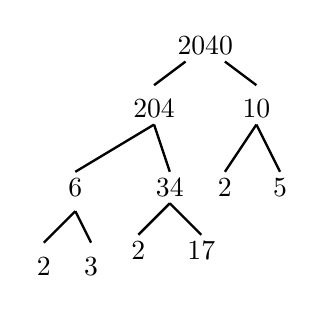
\begin{tikzpicture}
	\node at (-0.15,0) {$2040$};
	\draw[line width=0.03cm] (-0.4,-0.2) -- (-0.8,-0.5);
	\node at (-0.8,-0.8) {$204$};
	\draw[line width=0.03cm]  (0.1,-0.2) -- (0.5,-0.5);
	\node at (0.5,-0.8) {$10$};
		
	\draw[line width=0.03cm] (-0.8,-1) -- (-1.8,-1.6);
	\node at (-1.8,-1.8) {$6$};
	\draw[line width=0.03cm] (-0.8,-1) -- (-0.6,-1.6);
	\node at (-0.6,-1.8) {$34$};
	
	\draw[line width=0.03cm] (0.5,-1) -- (0.1,-1.6);
	\node at (0.1,-1.8) {$2$};
	\draw[line width=0.03cm] (0.5,-1) -- (0.8,-1.6);
	\node at (0.8,-1.8) {$5$};
	
	\draw[line width=0.03cm] (-2.2, -2.5) -- (-1.8, -2.1);
	\node at (-2.2,-2.8) {$2$};
	\draw[line width=0.03cm] (-1.6,-2.5) -- (-1.8, -2.1);
	\node at (-1.6,-2.8) {$3$};
	
	\draw[line width=0.03cm] (-0.2, -2.4) -- (-0.6,-2.0);
	\node at (-0.2,-2.6) {$17$};
	\draw[line width=0.03cm] (-1.0,-2.4) -- (-0.6,-2.0);
	\node at (-1.0,-2.6) {$2$};
	\end{tikzpicture}
	\] 
Therefore, the prime factorization of 2040 is $2040= 2^3 \cdot 3 \cdot 5 \cdot 17$. \pspace

\item We know that if $a= \prod_i p_i^{a_i}$ and $b= \prod_i p_i^{b_i}$, where the $p_i$ are prime and $a_i, b_i \geq 0$, then $\gcd(a, b)= \gcd \left( \prod_i p_i^{a_i}, \prod_i p_i^{b_i} \right)= \prod_i p^{\min(a_i, b_i)}$. But then we have\dots
	\[
	\gcd(2^{173} \cdot 3^{187} \cdot 5^{685} \cdot 11^{203}, \; 2^{578} \cdot 3^{281} \cdot 7^{323} \cdot 13^{360})= 2^{173} \cdot 3^{187}
	\]
Any divisors of two positive integers $a, b$ divides the $\gcd(a, b)$. But then if $\gcd(a, b)= \prod_i p_i^{g_i}$, where the $p_i$ are prime and $g_i \geq 0$, any divisor of $a, b$ must be of the form $\prod_i p_i^{d_i}$, where $0 \leq d_i \leq g_i$. Assuming $\gcd(a, b) > 1$, the next greatest divisor must have the same prime factorization as $\gcd(a, b)$ with one less power of the smallest prime divisor of $\gcd(a, b)$ with nonnegative power. Applying this in the case above, the next largest divisor is $2^{172} \cdot 3^{187}$. 


\item We know that if $a= \prod_i p_i^{a_i}$ and $b= \prod_i p_i^{b_i}$, where the $p_i$ are prime and $a_i, b_i \geq 0$, then $\lcm(a, b)= \lcm \left( \prod_i p_i^{a_i}, \prod_i p_i^{b_i} \right)= \prod_i p^{\max(a_i, b_i)}$. But then we have\dots
	\[
	\lcm(2^{173} \cdot 3^{187} \cdot 5^{685} \cdot 11^{203}, \; 2^{578} \cdot 3^{281} \cdot 7^{323} \cdot 13^{360})= 2^{578} \cdot 3^{281} \cdot 5^{686} \cdot 7^{323} \cdot 11^{203} \cdot 13^{360}
	\]
Any multiple of two positive integers $a, b$ must be a multiple of $\lcm(a, b)$. But then if $\lcm(a, b)= \prod_i p_i^{\ell_i}$, where the $p_i$ are prime and $\ell_i \geq 0$, any divisor of $a, b$ must be of the form $\prod_i p_i^{d_i}$, where $g_i \leq \ell_i$. But then the next smallest multiple must have the same prime factorization as $\lcm(a, b)$ with one additional power of the smallest possible prime---namely, 2. Applying this in the case above, the next smallest multiple is $2^{579} \cdot 3^{281} \cdot 5^{686} \cdot 7^{323} \cdot 11^{203} \cdot 13^{360}$.
\end{enumerate}
}



% Question 7
\newpage
\question[10] Showing all your work, compute the following:
	\begin{enumerate}[(a)]
	\item $(2468 \cdot 3579 + 97531) \mmod 2$
	\item $(10 - 18)^{100} \mmod 3$
	\item $(3^{11} + 3^{10}) \mmod 4$
	\item $(16 \cdot -7) \mmod 5$
	\item $(-17 \cdot 13 + 145) \mmod 6$
	\end{enumerate} \pspace

\sol {\itshape
\begin{enumerate}[(a)]
\item 
	\[
	(2468 \cdot 3579 + 97531) \equiv 0 \cdot 1 + 1 \equiv 0 + 1 \equiv 1 \mmod 2
	\] \pspace

\item  
	\[
	(10 - 18)^{100} \equiv (-8)^{100} \equiv 1^{100} \equiv 1 \mmod 3
	\] \pspace

\item  
	\[
	(3^{11} + 3^{10}) \equiv 3^{10} (3 + 1) \equiv 3^{10} \cdot 4 \equiv 3^{10} \cdot 0 \equiv 0 \mmod 4
	\] \pspace

\item  
	\[
	16 \cdot -7  \equiv 1 \cdot 3 \equiv 3 \mmod 5
	\] \pspace

\item  
	\[
	-17 \cdot 13 + 145 \mmod 1 \cdot 1 + 1 \equiv 1 + 1 \equiv 2 \mmod 6
	\] 
\end{enumerate}
}



% Question 8
\newpage
\question[10] Being sure to show all your work and fully explaining your logic, complete the following:
	\begin{enumerate}[(a)]
	\item What is the remainder when $2022^{2024}$ is divided by $2023$?
	\item What are the last three digits of $2022^{50}$?
	\item Show that working modulo two that $(x + y)^2= x^2 + y^2$. 
	\end{enumerate} \pspace

\sol {\itshape 
\begin{enumerate}[(a)]
\item The remainder when $2022^{2024}$ is divided by $2023$ is $2022^{2024} \mmod 2023$. We have\dots
	\[
	2022^{2024} \equiv (-1)^{2024} \equiv 1 \mmod 2023
	\]
Therefore, the remainder when $2022^{2024}$ is divided by $2023$ is 1. \pspace

\item The last three digits of $2022^{50}$ is the remainder when $2022^{50}$ is divided by 1000. But this is precisely $2022^{50} \mmod 1000$. Observe\dots
	\[
	\begin{aligned}
	2022^1&\equiv 22 \mmod 1000 \\
	2022^2&\equiv (2022^1)^2 \equiv 22^2 \equiv 484 \mmod 1000 \\
	2022^4&\equiv (2022^2)^2 \equiv 484^2 \equiv 234256 \equiv 256 \mmod 1000 \\
	2022^8&\equiv (2022^4)^2 \equiv 256^2 \equiv 65536 \equiv 536 \mmod 1000 \\
	2022^{16}&\equiv (2022^8)^2 \equiv 536^2 \equiv 287296 \equiv 296 \mmod 1000 \\
	2022^{32}&\equiv (2022^{16})^2 \equiv 296^2 \equiv 87616 \equiv 616 \mmod 1000
	\end{aligned}
	\]
Observe that $50= 32 + 16 + 2$. But then\dots
	\[
	\hspace{-3cm} 2022^{50} \equiv 2022^{32 + 16 + 2} \equiv 2022^{32} \cdot 2022^{16} \cdot 2022^2 \equiv 616 \cdot 296 \cdot 484 \equiv 182336 \cdot 484 \equiv 336 \cdot 484 \equiv 162624 \equiv 624 \mmod 1000
	\] \pspace

\item Observe that working modulo 2, we have\dots
	\[
	(x + y)^2= (x + y)(x + y)= x^2 + xy + yx + y^2= x^2 + xy + xy + y^2= x^2 + 2xy + y^2 \equiv x^2 + y^2 \mmod 2
	\]
\end{enumerate}
}



% Question 9
\newpage
\question[10] Let $a= 1561$ and $b= 8525$.
	\begin{enumerate}[(a)]
	\item Use the Euclidean algorithm to find $\gcd(a, b)$. 
	\item Explain why $a^{-1}$ exists $\mmod b$.
	\item Continuing your work in (a), use the extended Euclidean algorithm to compute $a^{-1}$ mod 8525.
	\item Prove that your answer in (c) is correct. 
	\end{enumerate} \pspace

\sol {\itshape
\begin{enumerate}[(a)]
\item Repeatedly applying the division algorithm with $b= 8525$ and $a= 1561$ and using the fact that $a> 0$, we have\dots
	\[
	\begin{aligned}
	8525&= 5(1561) + 720; & q& = \floor*{\dfrac{8525}{1561}}= 5, & r& = 8525 - 5(1561)= 8525 - 7805= 720 \\
	1561&= 2(720) + 121; & q& = \floor*{\dfrac{1561}{720}}= 2, & r&= 1561 - 2(720)= 1561 - 1440= 121 \\
	720&= 5(121) + 115; & q& = \floor*{\dfrac{720}{151}}= 5, & r&= 720 - 5(121)= 720 - 605= 115 \\
	121&= 1(115) + 6; & q& = \floor*{\dfrac{121}{115}}= 1, & r&= 121 - 1(115)= 121 - 115= 6 \\
	115&= 19(6) + 1; & q& = \floor*{\dfrac{115}{6}}= 19, & r&= 115 - 19(6)= 115 - 114= 1 \\
	6&= 6(1) + 0; & q& = \floor*{\dfrac{6}{1}}= 6, & r&= 6 - 6(1)= 6 - 6= 0 
	\end{aligned}
	\]
Therefore, $\gcd(1561, 8525)= 1$. \pspace

\item We know that $a^{-1}$ exists modulo $N$ if and only if $\gcd(a, N)= 1$. Using (a), we know $\gcd(1561, 8525)= 1$. Therefore, $1561^{-1}$ exists modulo 8525. \pspace

\item Using the extended algorithm, we can write $1561x + 8525y= \gcd(1561, 8525)= 1$ for some $x, y$. But taking this equation modulo 8525, we have $1561x \equiv 1 \mmod 8525$. But then $1561^{-1} \equiv x \mmod 8525$. \pspace

\item First, solving for the remainders, we have\dots
	\[
	\begin{aligned}
	1&= 115 - 19(6) \\
	6&= 121 - 1(115) \\
	115&= 720 - 5(121) \\
	121&= 1561 - 2(720) \\
	720&= 8525 - 5(1561)
	\end{aligned}
	\]
But then using the extended Euclidean algorithm, we have\dots
	\[
	\begin{aligned}
	1&= 115 - 19(6) \\
	&= 115 - 19 \big(121 - 1(115) \big)= 115 - 19 \cdot 121 + 19 \cdot 115= 20 \cdot 115 - 19 \cdot 121 \\
	&= 20 \big(720 - 5(121) \big) - 19 \cdot 121= 20 \cdot 720 - 100 \cdot 121 - 19 \cdot 121= 20 \cdot 720 - 119 \cdot 121 \\
	&= 20 \cdot 720 - 119 \big(1561 - 2(720) \big)= 20 \cdot 720 - 119 \cdot 1561 + 238 \cdot 720= 258 \cdot 720 - 119 \cdot 1561 \\
	&= 258 \big(8525 - 5(1561) \big) - 119 \cdot 1561= 258 \cdot 8525 - 1290 \cdot 1561 - 119 \cdot 1561 \\
	&= -1409 \cdot 1561 + 258 \cdot 8525 
	\end{aligned}
	\]
Taking this equation modulo 8525, we have $-1409 \cdot 1561 \equiv 1 \mmod 8525$. But then $-1409 \equiv 7116 \mmod 8525$ is the inverse of 1561 modulo $8525$, i.e. $1561^{-1} \equiv 7116 \mmod 8525$. \pspace

\item The inverse of an element $a \mmod N$ is an element $b \mmod N$ such that $ab \equiv 1 \mmod N$. The inverse, when it exists, is unique. Therefore, we only need check that $1561 \cdot 7116 \equiv 1 \mmod 8525$. This is routine:
	\[
	1561 \cdot 7116 \equiv 11108076 \equiv 1303(8525) + 1 \equiv 1 \mmod 8525
	\]
\end{enumerate}
}



% Question 10
\newpage
\question[10] Solve the following system of congruences and show that your solution is correct:
	\[
	\begin{cases}
	x + 1 \equiv 2 \mmod 3 \\
	x \equiv 0 \mmod 5 \\
	3x + 4 \equiv 2 \mmod 7 \\
	1 - x \equiv 4 \mmod 11
	\end{cases}
	\] \pspace

\sol {\itshape First, we put each congruence into the form $x \equiv a_i \mod m_i$. 

	\[
	\begin{aligned}
	x + 1&\equiv 2 \mmod 3 &\quad x&\equiv 0 \mmod 5 &\quad 3x + 4&\equiv 2 \mmod 7 &\quad 1 - x&\equiv 4 \mmod 11 \\
	x&\equiv 1 \mmod 3 & x&\equiv 0 \mmod 5 & 3x&\equiv -2 \mmod 7 & 1&\equiv x + 4 \mmod 11 \\
	& & & & 3x&\equiv 5 \mmod 7 & x&\equiv -3 \mmod 11 \\
	& & & & 3^{-1} \cdot 3x&\equiv 3^{-1} \cdot 5 \mmod 7 & x&\equiv 8 \mmod 11 \\
	& & & & x&\equiv 5 \cdot 5 \mmod 7 \\
	& & & & x&\equiv 25 \mmod 7 \\
	& & & & x&\equiv 4 \mmod 7 \\
	\end{aligned}
	\]
Therefore, this system of congruences is equivalent to the following system of congruences:
	\[
	\begin{cases}
	x \equiv 1 \mmod 3 \\
	x \equiv 0 \mmod 5 \\
	x \equiv 4 \mmod 7 \\
	x \equiv 8 \mmod 11
	\end{cases}
	\] 
Because $\gcd(3, 5, 7, 11)= 1$, the Chinese Remainder Theorem states that there is a solution, which is unique modulo $M:= 3 \cdot 5 \cdot 7 \cdot 11= 1155$. The solution(s) have the same residue class as $x= \sum a_i N_i M_i$, where $M_i= M/m_i$ and $N_i= M_i^{-1} \mmod m_i$. From the work above, we have\dots
	\[
	\begin{aligned}
	a_1&= 1 \\
	a_2&= 0 \\
	a_3&= 4 \\
	a_4&= 8
	\end{aligned}
	\]
Furthermore, we have\dots
	\[
	\begin{aligned}
	M_1&= \dfrac{M}{m_1}= \dfrac{1155}{3}= 5 \cdot 7 \cdot 11= 385 \\
	M_2&= \dfrac{M}{m_2}= \dfrac{1155}{5}= 3 \cdot 7 \cdot 11= 231 \\
	M_3&= \dfrac{M}{m_3}= \dfrac{1155}{7}= 3 \cdot 5 \cdot 11= 165 \\
	M_4&= \dfrac{M}{m_4}= \dfrac{1155}{11}= 3 \cdot 5 \cdot 7= 105
	\end{aligned}
	\]
Now we need compute $N_i= M_i^{-1} \mod m_i$. First, we reduce each $M_i$ modulo $m_i$:
	\[
	\begin{aligned}
	M_1&= 385 \equiv 1 \mmod 3 \\
	M_2&= 231 \equiv 1 \mmod 5 \\
	M_3&= 165 \equiv 4 \mmod 7 \\
	M_4&= 105 \equiv 6 \mmod 11
	\end{aligned}
	\]
Clearly, $N_1= M_1^{-1} \mmod 3= 1^{-1} \mmod 3= 1 \mmod 3$. Similarly, we know $N_2= M_2^{-1} \mmod 5= 1^{-1} \mmod 5= 1 \mmod 5$. To compute $N_3= M_3^{-1} \mmod 7= 4^{-1} \mmod 7$. But because $4 \cdot 2= 8 \equiv 1 \mmod 7$, we know that $N_3= 4^{-1} \equiv 2 \mmod 7$. Finally, we need to compute $N_4= M_4^{-1} \mmod 11= 6^{-1} \mmod 11$. But because $6 \cdot 2= 12 \equiv 1 \mmod 11$, we know that $N_4= 6^{-1} \equiv 2 \mmod 11$. Therefore, we have\dots
	\[
	\begin{aligned}
	N_1&= 1 \\
	N_2&= 1 \\
	N_3&= 2 \\
	N_4&= 2
	\end{aligned}
	\]
But then the unique solution modulo $M= 3 \cdot 5 \cdot 7 \cdot 11= 1155$ is\dots
	\[
	\hspace{-0.75cm} \sum a_i N_i M_i= 1(1)385 + 0(1)231 + 4(2)165 + 8(2)105= 385 + 0 + 1320 + 1680= 3385 \equiv 1075 \mmod 1155
	\]
Therefore, the unique solution modulo 1155 is 1075 and the integer solutions are those integers $n$ such that $n \equiv 1075 \mmod 1155$, e.g. $-1235$, $-80$, $1075$, $2230$, $3385$, etc. 
}


\end{questions}
\end{document}